\documentclass[journal=jacsat,manuscript=article]{achemso}
\usepackage[version=3]{mhchem}
\usepackage{amsmath}
\usepackage{ctex}
\usepackage{longtable}
\usepackage{booktabs}
\newcommand*\mycommand[1]{\texttt{\emph{#1}}}
\providecommand{\tightlist}{%
  \setlength{\itemsep}{0pt}\setlength{\parskip}{0pt}}
\author{蓝海}
\altaffiliation{我们认真科学分析金融的规律}
\email{lh_loki@163.com}
\phone{13127900572}
\author{彭莉}


\keywords{成长, 防守进攻两端}

\title[申坤]{申坤简评\footnote{详尽的数据分析与记录请联系作者索取《基金管理人分析技术文档》}}
\makeatletter
\ifxetex
  \usepackage[setpagesize=false, % page size defined by xetex
              unicode=false, % unicode breaks when used with xetex
              xetex]{hyperref}
\else
  \usepackage[unicode=true]{hyperref}
\fi
\hypersetup{breaklinks=true,
            bookmarks=true,
            pdfauthor={},
            pdftitle={},
            colorlinks=true,
            urlcolor=blue,
            linkcolor=magenta,
            pdfborder={0 0 0}}
\urlstyle{same}  % don't use monospace font for urls
% pandoc header

\begin{document}
\begin{abstract}
申坤是市场上成长股投资的刚刚展露头角新星。在7年的证券行业从业经历中,以基金经理人的身份长期管理两只基金,一只自2015年股灾时接手到现在基本盈亏相当,另外一只自2016年4月接手,到现在取得了50\%的回报,共管理34.26亿元的资金。

基于公开信息分析,我们认为申坤是典型的成长股、相当集中型投资者。交易风格为中高换手、高集中度。这样风格的投资这在当前的市场环境还能取得如此亮眼的成绩得益于其具备较强的选股能力、择时能力和中等的行业配置能力,长期保持积极的主动投资。
\end{abstract}
\begin{figure}[htbp]
\centering
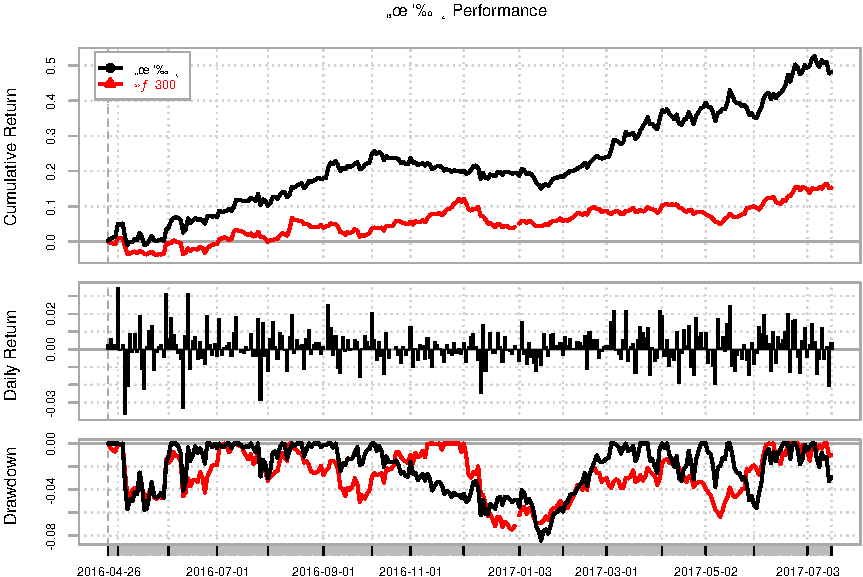
\includegraphics{sk-review_files/figure-latex/unnamed-chunk-2-1.pdf}
\caption{基金累计回报率与回撤}
\end{figure}

\begin{longtable}[]{@{}llclclc@{}}
\toprule
名称 & 近半年 & 夏普率 & 近一年 & 夏普率 & 近两年 &
夏普率\tabularnewline
\midrule
\endhead
国泰金鑫 & 23.3\% & 3.0 & 39\% & 2.24 & 48\% & 2.13\tabularnewline
沪深300 & 8.9\% & 1.6 & 16\% & 0.85 & 15\% & 0.73\tabularnewline
\bottomrule
\end{longtable}

\begin{figure}[htbp]
\centering
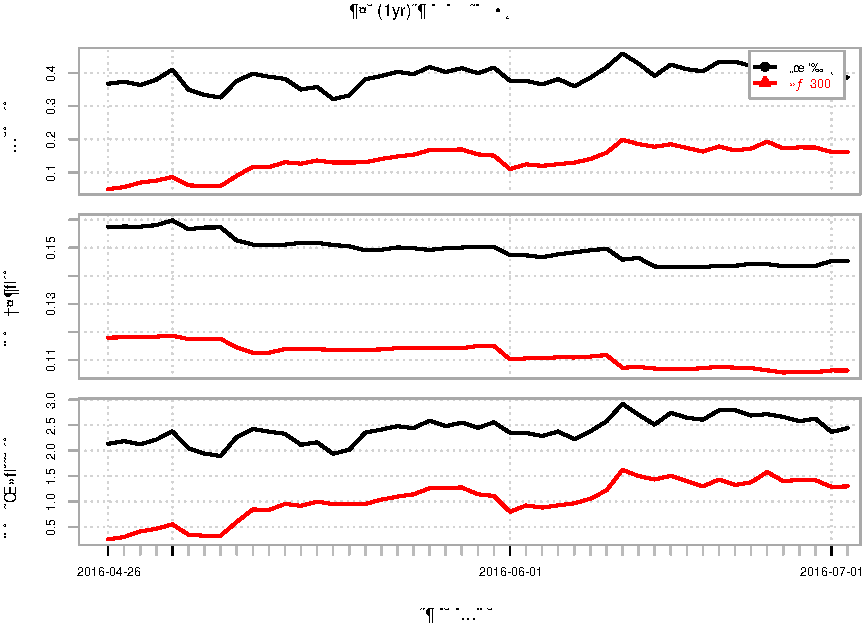
\includegraphics{sk-review_files/figure-latex/unnamed-chunk-3-1.pdf}
\caption{投资者收益风险比较}
\end{figure}

\section{简介}

女,硕士研究生。2010年4月加入国泰基金管理有限公司,历任消费品行业研究员、基金经理助理。2015年6月起任国泰成长优选混合型证券投资基金(原国泰成长优选股票型证券投资基金)的基金经理。

\section{风格评述}

申坤的风格集中表现为:

\begin{itemize}
\item 交易风格:中高换手率,高度股票与行业集中,当然如市场不好也会降低集中度和整体股票仓位
\item 持仓风格:中盘成长和小盘成长是主流配置,往往分别形成组合中的防守端和进攻端
\item 主动性风格:积极主动,主动指数为32\%。
\end{itemize}

\section{\texorpdfstring{能力评价\footnote{运气能够带来超常表现,持续的好运则可以归结为能力!}}{能力评价}}

我们讲持续的超额表现归因为

\begin{equation}
\mbox{大类资产配置能力} + \mbox{行业配置能力(股票类)}+ \mbox{择股能力} + \mbox{择时能力} \Rightarrow \mbox{超额收益}
\end{equation}

\begin{table}
  \begin{tabular}{l|llll}
    因子 &大类资产配置  & 行业配置  & 择股能力 & 择时能力  \\ \hline
    贡献收益 & $-0.6\%$   & $3.69\%$ & $11.92\%$ &  $12,73\%$  \\
    评价 & 无 & 中等 & 较强 & 突出\footnote{排除股灾时期表现}  \\ \hline
  \end{tabular}
\end{table}

\section{投资策略简述}

\subsection{进攻防守两端论}

一个投资组合就像一个足球对,需要讲究攻守平衡:

\begin{itemize}
\tightlist
\item
  进攻端选择:小市值(往往也伴随高估值)如:消费电子、新能源
\end{itemize}

\begin{longtable}[]{@{}ll@{}}
\toprule
盈利增长  & PE\tabularnewline
\midrule
\endhead
50\% & 35-40\tabularnewline
30\% & 20-25\tabularnewline
\bottomrule
\end{longtable}

\begin{itemize}
\item
  防守端选择:稳定性强,同时有30\%左右增长,PE在20-25之间的二线白马,不配千亿以上``大白马''。如:家电、家居、食品、饮料
\item
  风控方法:随着市场的变化调整持股集中度和股票仓位;选择股票是充分考虑安全边际。
\end{itemize}

\section{评价}

申坤是新锐的成长股基金管理人。我们基于公开信息,进行深度的科学分析,结合与其面对面的交流,做出如下评判:

\begin{enumerate}
\def\labelenumi{\arabic{enumi}.}
\tightlist
\item
  申坤有高换手、集中持股的交易风格,和在``二线白马''和小盘成长之间进行攻守组合的投资风格,超高行业的集中度她看起来像是一个主题投资者;
\item
  申坤股票仓位调节是随着市场变化而采取的被动式的风控行为,因此没有表现出大类资产配置的能力;
\item
  作为一名消费品行业研究员出身的投资经理,把中观的行业层面融入到择股决策中,加之个股与行业的集中度都很高,因而体现出了中等的行业配置能力;
\item
  作为成长股、周期股的投资人和高换手表现的投资选手,择时能力是她追寻的投资回报的主要手段之一,比如它的进攻防守两端论中,进攻端的选取与卖出依赖因较强的择时能力。在她过去两年的投资管理中,除了灾难性市场表现一般之外,在大多数时候,申坤都表现除了突出的择时能力;
\item
  择股能力是最为重要的盈利手段,申坤在该项目上表现了较强的能力。
\end{enumerate}

因此,申坤是适合中期投资的、成长股领域内的、积极的基金管理人。

\begin{acknowledgement}

在我们的分析中,使用了公开数据与部分非公开数据,在此基础上采用基于净值的风格分析,基于持仓的收益归因对基金管理人的业绩表现进行了科学的分析。我们历尽所能的使用了最为完整与详实的数据、最为科学的方法,以最为严谨的态度做出尽量客观的评价。同时我们也实地进行调研与基金经理人进行了多次的交流。在此,对于向我们提供数据与交流机会的相关人员致谢。需要根伟详细的技术分析报告,请与本文作者联系。

\end{acknowledgement}
\end{document}
